%%%%%%%%%%%%%%%%%%%%%%%%%%%%%%%%%%%%%%%%%%%%%%%%%%%%%%%%%%%%%%%%%%%%%
%
% CSCI 1430 Written Question Template
%
% This is a LaTeX document. LaTeX is a markup language for producing documents. 
% You will fill out this document, compile it into a PDF document, then upload the PDF to Gradescope. 
%
% To compile into a PDF on department machines:
% > pdflatex thisfile.tex
%
% If you do not have LaTeX, your options are:
% - Personal laptops (all common OS): http://www.latex-project.org/get/ 
% + VSCode extension: https://marketplace.visualstudio.com/items?itemName=James-Yu.latex-workshop
% - Online Tool: https://www.overleaf.com/ - most LaTeX packages are pre-installed here (e.g., \usepackage{}).
%
% If you need help with LaTeX, please come to office hours.
% Or, there is plenty of help online:
% https://en.wikibooks.org/wiki/LaTeX
%
% Good luck!
% The CSCI1430 staff
%
%%%%%%%%%%%%%%%%%%%%%%%%%%%%%%%%%%%%%%%%%%%%%%%%%%%%%%%%%%%%%%%%%%%%%

\documentclass{csci1430}

\begin{document}
\title{Homework 1 Written Questions}
\maketitle
\thispagestyle{fancy}

\writeinstructions

\section*{This Homework}
\begin{itemize}
    \item 6 questions \textbf{[12 + 8 + 6 + 7 + 14 + 7 = 54]}.
    \item Include code, images, and equations where appropriate.
\end{itemize}

% Please leave the pagebreak
\pagebreak
%%%%%%%%%%%%%%%%%%%%%%%%%%%%%%%%%%%%%%%%%%%

\begin{question}[points=12,drawbox=false]
We have been given special permission to use the telescope on the roof of Barus and Holley. Unfortunately, our fantastic image of the Orion nebula has noise: (\href{run:images/orion-noise.png}{orion-noise.png})

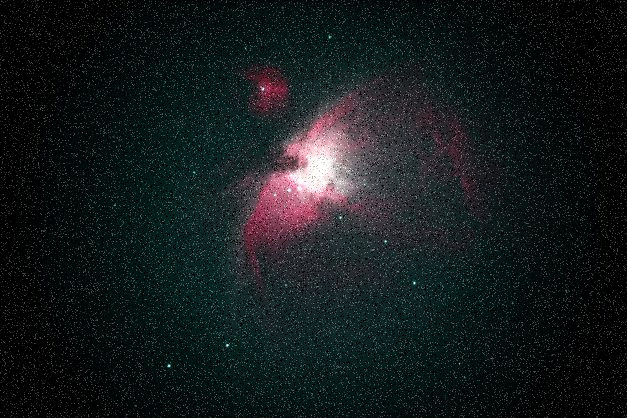
\includegraphics[width=0.5\textwidth,height=6cm,keepaspectratio]
{images/orion-noise.png}

One way to deal with this noise is with image convolution.
Convolution is a type of image filtering that is a fundamental image processing tool.
\end{question}

\begin{orangebox}
\emph{Explicitly describe} the input, transformation, and output components of 2D discrete convolution. Please be precise; define variables as need.
\end{orangebox}

\begin{subsubquestion}[points=2]
Input \textbf{[2--4 sentences]}
\end{subsubquestion}

\begin{answer}[height=7]

\end{answer}

\begin{subsubquestion}[points=2]
    Transformation (how is the image transformed?) \textbf{[2--4 sentences]}
\end{subsubquestion}

\begin{answer}[height=9]

\end{answer}

\pagebreak    
\begin{subsubquestion}[points=2]
    Output \textbf{[2--4 sentences]}
\end{subsubquestion}

\begin{answer}[height=7]

\end{answer}


\begin{subquestion}[points=4]
Describe two filter kernels that we may use with convolution, and give an example computer vision application that each enables. \textbf{[4--8 sentences]}
\end{subquestion}

\begin{answer}[height=14]

\end{answer}

\begin{subquestion}[points=2]
What kind of filter might we use to de-noise our image of the Orion nebula, and why? \textbf{[2--3 sentences]}
\end{subquestion}

\begin{answer}[height=7]

\end{answer}

\pagebreak
% %%%%%%%%%%%%%%%%%%%%%%%%%%%%%%%%%%%

\begin{question}[points=8,drawbox=false]
Now that we've de-noised our image of the Orion nebula, let's explore filtering techniques more closely. Two kinds of linear filtering are correlation and convolution.
\end{question}

\begin{subquestion}[points=3]
    What is different between convolution and correlation? Include differences in their algebraic properties. When might we use each? \textbf{[5--6 sentences]}
\end{subquestion}    
    
\begin{answer}[height=14]
    
\end{answer}
    
To solidify our understanding of the distinction between correlation and convolution, we will process another image.
    
\begin{subquestion}[points=4]
    Devise a scenario in which the output of correlation and convolution differ.
    
    Write code that loads an image and produces two distinct images, one from convolution and one from correlation on some kernel of your choice. Then, compute the difference of the two images (the order in which you subtract the images should not matter) and display it as well.
    
    Specify your kernel, and provide the input image and two output results. Then, use your understanding of convolution and correlation to explain the outputs. \textbf{[2--4 sentences]}
\end{subquestion}
    
\emph{Consider \href{https://docs.scipy.org/doc/scipy/reference/generated/scipy.signal.convolve2d.html}{$scipy.signal.convolve2d$} and \href{https://docs.scipy.org/doc/scipy/reference/generated/scipy.signal.correlate2d.html}{$scipy.signal.correlate2d$} to experiment!}
    

\begin{answer}
    
\includegraphics[width=0.5\textwidth,height=7cm,keepaspectratio]{images/TODO_orig_img.png}
    
\includegraphics[width=0.5\textwidth,height=7cm,keepaspectratio]{images/TODO_difference.png}\\
    
\includegraphics[width=0.5\textwidth,height=7cm,keepaspectratio]{images/TODO_conv_res.png}
    
\includegraphics[width=0.5\textwidth,height=7cm,keepaspectratio]{images/TODO_corr_res.png}
    
    TODO: Your explanation here.
\end{answer}

\pagebreak

\begin{subquestion}[points=1]
Consider a situation where we apply two different filters sequentially to an image. How will the output image change depending on the order in which we apply the filters? Will the behavior be different for convolution versus correlation? \textbf{[1--2 sentences]}
\end{subquestion}

\begin{answer}[height=14]
    
\end{answer}

\pagebreak % Please leave the page break
% %%%%%%%%%%%%%%%%%%%%%%%%%%%%%%%%%%%

\begin{question}[points=6,drawbox=false]
While exploring Brown CS's history in the halls of CIT, we happen upon Nancy: a DEC VAX 11/780. So struck by its beauty, we decide to take an artful photo with our camera. Modern digital sensors have many megapixels, so we resize it to make the file smaller.

\begin{tabular}{c c}
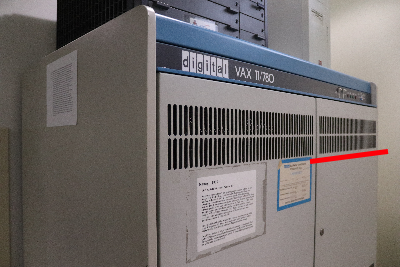
\includegraphics[width=0.49\textwidth,height=7cm,keepaspectratio]{images/poor_nancy_markup.png} &
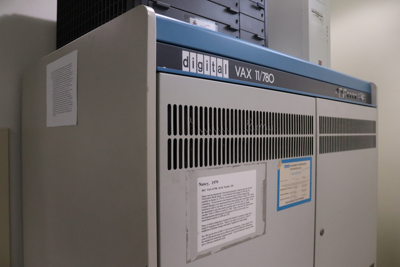
\includegraphics[width=0.49\textwidth,height=7cm,keepaspectratio]{images/poor_nancy_better.png} \\
Resized image & Depiction of original (\emph{not original file})
\end{tabular}

Oh no! What happened to Nancy? There are weird artifacts in the vents (above red line)---these definitely weren't there in the original photo. Plus, if we look closely, the white label text is less smooth and there are jagged lines.
\end{question}

\begin{subquestion}[points=3]
What is this phenomenon called, and why did it happen? \textbf{[2--4 sentences]}
\end{subquestion}

\begin{answer}[height=8]

\end{answer}

\begin{subquestion}[points=3]
How might we fix this issue with filtering? Describe the process, and explain why it works. \textbf{[2--4 sentences]}
\end{subquestion}

\begin{answer}[height=8]

\end{answer}

\pagebreak % Please leave the page break
% %%%%%%%%%%%%%%%%%%%%%%%%%%%%%%%%%%%

\begin{question}[points=7,drawbox=false]
With filtering, we can remove different frequencies of information from an image, or let them `pass through' to the output. Which kind of filter produced these outputs?
\end{question}

\raisebox{\baselineskip-\height}{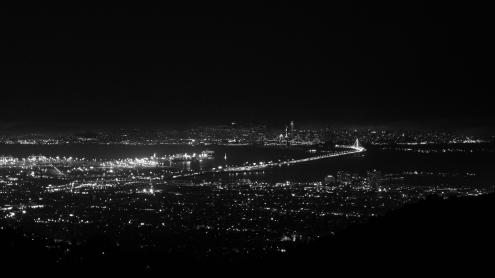
\includegraphics[width=0.5\textwidth,height=7cm,keepaspectratio]{images/q3img0.png}}

\begin{subsubquestion}[points=2]
Output image 1:\\
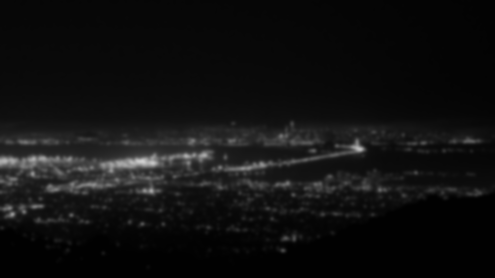
\includegraphics[width=0.6\textwidth,height=7cm,keepaspectratio]{images/q3img1.png}
\end{subsubquestion}

\begin{answerlist}
% Remember: use \item[\done] to mark an answer.
    \item High pass
    \item Low pass
\end{answerlist}

\begin{subsubquestion}[points=2]
Output image 2 (adjusted for easier visualization):\\
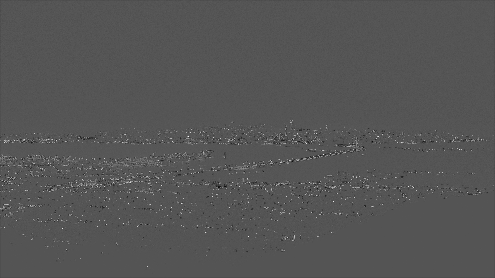
\includegraphics[width=0.6\textwidth,height=7cm,keepaspectratio]{images/q3img2.png}
\end{subsubquestion}

\begin{answerlist}
    \item High pass
    \item Low pass
\end{answerlist}

\pagebreak

\begin{subquestion}[points=3]
Which of the following kernels is high pass, low pass, or neither?
\end{subquestion}

\emph{Note:} To fill in boxes, replace `\textbackslash square' with `\textbackslash blacksquare' for your answer.

\begin{enumerate}[(i)]
\item
 $\begin{bmatrix}
    1 & 0 & -1 \\
    1 & 0 & -1 \\
    1 & 0 & -1 \\
 \end{bmatrix}$

\begin{answerlist}
    % Remember: use \item[\done] to mark an answer.
    \item High pass
    \item Low pass
    \item Neither
\end{answerlist}

\item
 $\begin{bmatrix}
    \frac{1}{9} & \frac{1}{9} & \frac{1}{9} \\
    \frac{1}{9} & \frac{1}{9} & \frac{1}{9} \\
    \frac{1}{9} & \frac{1}{9} & \frac{1}{9}
 \end{bmatrix}$

 \begin{answerlist}
    % Remember: use \item[\done] to mark an answer.
    \item High pass
    \item Low pass
    \item Neither
\end{answerlist}

\item
$\begin{bmatrix}
    -\frac{1}{9} & -\frac{1}{9} & -\frac{1}{9} \\
    -\frac{1}{9} & \frac{8}{9} & -\frac{1}{9} \\
    -\frac{1}{9} & -\frac{1}{9} & -\frac{1}{9}
\end{bmatrix}$

\begin{answerlist}
    % Remember: use \item[\done] to mark an answer.
    \item High pass
    \item Low pass
    \item Neither
\end{answerlist}

\end{enumerate}

\pagebreak

\begin{subquestion}[points=2]
Which of the following statements are true?
\end{subquestion}

\begin{answerlist}
\item High pass filter kernels will always contain at least one negative number
\item A Gaussian filter is an example of a low pass filter
\item A high pass filter is the basis for most smoothing methods
\item In a high pass filter, the center of the kernel must have the highest value
\end{answerlist}


\pagebreak
%%%%%%%%%%%%%%%%%%%%%%%%%%%%%%%%%

\begin{question}[points=14,drawbox=false]
With filtering, we can create \emph{hybrid images} that depict different objects when viewed at different distances. They are inauthentic images of the natural world.

As technology advances, evaluating the authenticity of images becomes increasingly difficult. Please read \href{https://www.nytimes.com/1990/08/12/arts/photography-view-ask-it-no-questions-the-camera-can-lie.html}{this article} by photography critic Andy Grundberg in the \emph{New York Times} from August 1990.

Grundberg stated that: ``In the future, readers of newspapers and magazines will probably view news pictures more as illustrations than as reportage, since they can no longer distinguish between a genuine image and one that has been manipulated.''
\end{question}

\begin{subquestion}[points=4]
When is Grundberg's future, and why? \textbf{[4--6 sentences]}
\end{subquestion}

\begin{answer}[height=11]

\end{answer}

\begin{subquestion}[points=4]
For a news picture, are any digital manipulations permissible? If so, how do we decide which ones? Use at least one ethical framework from the \href{https://browncsci1430.github.io/resources/ethics_primer/}{ethics primer} to explore this. \textbf{[4--6 sentences]}
\end{subquestion}

\begin{answer}[height=11]

\end{answer}
    
\pagebreak

The Coalition for Content Provenance and Authenticity (C2PA) has designed a technical specification to attach history to an image. Please watch \href{https://www.youtube.com/watch?v=hA0ZjqakEF8}{this video} for an overview; stop at 4 minutes and 40 seconds.

For context, a stakeholder of a system is identified as a person or group who has an explicit interest or concern in the system itself, its operations, and its consequences.
    
\begin{subquestion}[points=4]
Describe one situation in which the C2PA system helps us in determining authenticity and identify one stakeholder that benefits. Then, describe a second situation in which C2PA does not help to determine authenticity and one stakeholder that is still at risk. Please explain why C2PA helps or not in each case. \textbf{[4--6 sentences]}
\end{subquestion}

\begin{answer}[height=12]

\end{answer}

\begin{subquestion}[points=2]
Grundberg's article is titled ``Ask It No Questions: The Camera Can Lie.''

Does the C2PA system weaken Grundberg's argument? \textbf{[1--2 sentences]}
\end{subquestion}

\begin{answer}[height=8]

\end{answer}

\pagebreak
% %%%%%%%%%%%%%%%%%%%%%%%%%%%%%%%%%%%

\begin{question}[points=7,drawbox=false]
\textbf{Technical practice.} In computer vision, each image is a matrix of pixels. The \texttt{numpy} library provides fast computation with large multi-dimensional vectors and matrices. 

To familiarize yourself with the library, read through the following scenarios and complete the exercises. Write \emph{one} \texttt{numpy} function to complete each of the following tasks.

With \texttt{numpy} imported as
\begin{verbatim}
    import numpy as np
\end{verbatim}
we can call functions with 
\begin{verbatim}
    np.function_name(<arguments>)
\end{verbatim}
Test out your answers by creating your own python program. Some functions you might find useful are \href{https://numpy.org/doc/stable/reference/generated/numpy.squeeze.html}{np.squeeze}, \href{https://numpy.org/doc/stable/reference/generated/numpy.expand_dims.html}{np.expand\_dims}, \href{https://numpy.org/doc/stable/reference/generated/numpy.clip.html}{np.clip}, \href{https://numpy.org/doc/stable/reference/generated/numpy.pad.html}{np.pad}, and \href{https://numpy.org/doc/stable/reference/generated/numpy.zeros.html}{np.zeros}.

Use operators like \texttt{[]} and \texttt{:}, but remember that each prompt can be completed with only \textit{one} function/operator shorthand.
\end{question}

\begin{subquestion}[points=1]
Create a black image \texttt{img} with all values in this matrix equal to 0, where \texttt{np.shape(img) == (320,640)}.
\end{subquestion}
    
\begin{answer}
\begin{python}
# TODO: Your expression here
\end{python}
\end{answer}
    
\begin{subquestion}[points=1]
Assume we have a 2D matrix \texttt{img} with values range [-1.0, 1.0]. Clip \texttt{img} so that all its values lie within the range [-0.5, 0.5].
\end{subquestion}

\begin{answer}
\begin{python}
# TODO: Your expression here
\end{python}
\end{answer}

\pagebreak

\begin{subquestion}[points=1]
A malformed filter operation has messed up the output dimensions, producing a variable \texttt{img\_out} where \texttt{np.shape(img\_out) == (1, 1, 320, 640)}. Remove all 1-sized dimensions. Convert \texttt{img\_out} to a new matrix \texttt{img\_fixed} where \texttt{np.shape(img\_fixed) == (320, 640)}.
\end{subquestion}

\begin{answer}
\begin{python}
# TODO: Your expression here
\end{python}
\end{answer}

Color images are represented with a three dimensional matrix, where often the third dimension represents spectral information. The presence of a third dimension or the size of the color dimension could help us to identify whether an image is color (RGB) or grayscale.

\begin{subquestion}[points=1]
Say you have a grayscale image \texttt{img} where \texttt{np.shape(img) == (320, 640)}. Convert this to a new image \texttt{img\_expanded} where \texttt{np.shape(img\_expanded) == (320, 640, 1)}. In other words, add a 1-sized dimension to \texttt{img}.
\end{subquestion}

\begin{answer}
\begin{python}
# TODO: Your expression here
\end{python}
\end{answer}
    
\begin{subquestion}[points=1]
Suppose we have an RGB image matrix, \texttt{img}, of shape (320, 640, 3). Retrieve the third blue channel of the image while preserving all of \texttt{img}'s dimensions and intensity values.
\end{subquestion}
    
\begin{answer}
\begin{python}
# TODO: Your expression here
\end{python}
\end{answer}

\pagebreak

\begin{subquestion}[points=1]
Suppose we have a second RGB image matrix, \texttt{img2}, also of shape (320, 640, 3). Retrieve the red and blue channels of \texttt{img2} within a single variable of shape (320, 640, 2).
\end{subquestion}
    
\begin{answer}
\begin{python}
# TODO: Your expression here
\end{python}
\end{answer}
    
\begin{subquestion}[points=1]
Padding is a useful operation to help us produce a convolved image equal in size to an input image. Given an RGB image, \texttt{img} of (320, 640, 3), pad it with two columns of zeros on the left and right edges of the image, and three rows of zeros on the top and bottom edges of the image. Do not add zero padding to the color dimension.
\end{subquestion}
    
\begin{answer}
\begin{python}
# TODO: Your expression here
\end{python}
\end{answer}

\pagebreak
% %%%%%%%%%%%%%%%%%%%%%%%%%%%%%%%%%%%

\section*{Feedback? (Optional)}
We appreciate your feedback on how to improve the course. You can provide anonymous feedback through \href{https://forms.gle/Eu5jJbDUmLknAyJV9}{this form} which can be accessed using your Brown account (your identity will not be collected). If you have urgent non-anonymous comments/questions, please email the instructor. 

\end{document}
